\documentclass[12pt, twopage]{article}
\linespread{1.25}

\usepackage[utf8]{inputenc}
\usepackage{amsthm}
\usepackage[slovak]{babel}
\usepackage{graphicx}
\usepackage[hidelinks, breaklinks]{hyperref}

\theoremstyle{definition}
\newtheorem{example}{Príklad}

%[]

\title{\textbf{Rýchlokurz zlomkovej geniality\\}}
\date{}
\author{Roman Hudec\\
	\textit{Educat - vzdelávacie centrum}
}

\begin{document}
	\maketitle
	
	\begin{center}
		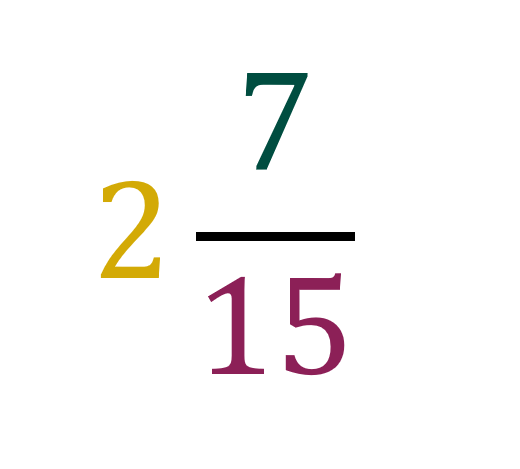
\includegraphics{zlomok.png}
	\end{center}
	
	\newpage
	\tableofcontents
	\newpage
	
	\section{Čo sú to zlomky}
	
	\subsection{Definícia zlomkov a racionálnych čísel}
	
	\subsection{Geometrické znázorňovanie zlomkov ako časti celku}
	
	\subsection{Znázorňovanie zlomkov na číselnej osi}
	
	\newpage
	\section{Matematické operácie so zlomkami}
	
	\subsection{Rozširovanie zlomku}
	
	\subsection{Krátenie zlomku}
	
	\subsection{Násobenie zlomkov}
	
	\subsection{Delenie zlomkov}
	
	\subsection{Sčitovanie zlomkov s rovankými menovateľmi}
	
	\subsection{Sčitovanie a odčitovanie zlomkov s rôznymi menovateľmi}
	
	\newpage
	\section{Ďalšie fičúry so zlomkami}
	
	\subsection{Zložený zlomok}
	
	\subsection{Zložené číslo}
	
	\subsection{Ako sú desatinné čísla a zlomky kamoši}
	
	\subsection{Čo má spoločné geometrické znázorňovanie zlomkov s ich rozširovaním a krátením}
	
	
\end{document}
